% ВАЖНО
% Не меняйте ничего в этом файле. А если меняете, то делайте это в этом проекте:
% https://github.com/kib-courses/latex_templates
% Для пользовательских настроек есть файл ./header/user.tex
\documentclass{beamer}
\usetheme{metropolis} 
\usecolortheme{rose}

\hypersetup{unicode=true}
\usepackage{tikz}

\usepackage{xcolor}
\usepackage[utf8]{inputenc}
\usepackage{hyphenat}
\usepackage[russian,english]{babel}          % Use metropolis theme
\usepackage{wrapfig}

\usepackage[normalem]{ulem}  % для зачекивания текста

\usepackage{caption}
\captionsetup[figure]{name=Рисунок }
\newcommand{\рис}[1]{рис.\ref{#1}}
\newcommand{\Рис}[1]{Рис.\ref{#1}}


\captionsetup[table]{name=Таблица~№}
\newcommand{\таблицa}[1]{таблица~№\ref{#1}} % именительный падеж
\newcommand{\таблицы}[1]{таблицы~№\ref{#1}} % родительный падеж
\newcommand{\таблице}[1]{таблице~№\ref{#1}} % дательный и предложный падеж
\newcommand{\таблицу}[1]{таблицу~№\ref{#1}} % винительный падеж
\newcommand{\таблицей}[1]{таблицей~№\ref{#1}} % творительный падеж 
\newcommand{\Таблицa}[1]{Таблица~№\ref{#1}} % именительный падеж
\newcommand{\Таблицы}[1]{Таблицы~№\ref{#1}} % родительный падеж
\newcommand{\Таблице}[1]{Таблице~№\ref{#1}} % дательный и предложный падеж
\newcommand{\Таблицу}[1]{Таблицу~№\ref{#1}} % винительный падеж
\newcommand{\Таблицей}[1]{Таблицей~№\ref{#1}} % творительный падеж 

\setbeamertemplate{footline}[frame number] % указывает на каждой странице общее количество страниц

% Указывайте все новые термины в \termdef команде. А уже известные ранее или из других курсов в \term
\newcommand{\termdef}[1]{\textbf{\textit{#1}}}
\newcommand{\term}{\textit}

% Диалог с аудиторией.
\newcommand{\auditorium}[1]{\textcolor{red}{\textbf{#1}}}

\let\OLDhref\href
\renewcommand{\href}[2]{\textcolor{blue}{\OLDhref{#1}{#2}}}

% \setbeameroption{show notes}
% \usepackage{listings}             % Include the listings-package
% \usepackage{minted}

\usepackage{CJKutf8}

\title{Лекция 5. Feature Extraction для текстовых данных и построение эффективных моделей}

% \date{\today}
\date{29 октября 2019}
\author{Павел Владимирович Слипенчук }
\institute{Москва, МГТУ им.Бауманка,\\ каф.ИУ-8, \href{https://t.me/kibinfo}{КИБ}}
% \titlegraphic{\includegraphics[width=2cm]{logo_ur.jpg}}
\titlegraphic{\small \href{https://github.com/kib-courses/dsis}{Data Science для решения задач информационной безопасности}}

\begin{document}
  \maketitle
    
\begin{frame}{План лекции}
    \begin{enumerate}
    	\item \nameref{section:fe}
		\item \nameref{section:neneural_network}
		\item \nameref{section:texts_fe1}
		\item \nameref{section:APTA}
		\item \nameref{section:texts_fe2}
	\end{enumerate}
\end{frame}

\section{Feature Extraction}\label{section:fe}

\begin{frame}{Процесс DS}
	Процесс DS:
	\begin{enumerate}
		\item Определение Д.Н.К. -- Дано, Найти, Критерий
		\item Получение row data
		\item \termdef{Feature Extraction}: Анализ row data, формирование гипотез, проверка гепотиз, автоматизация.
		\item Машинное обучение: создание прототипа модели на тестовых данных. Оценка качества системы
		\item Data Engeneering: создание DS системы в целом
		\item Машинное обучение: донастройка модели
		\item Внедрение
	\end{enumerate}
\end{frame}

\begin{frame}{Feature Extraction}
	\termdef{Feature Extraction} 
	(Извлечение признаков, выделение признаков) 
	-- это творческий процесс
	направленный на анализ данных (raw data),
	извлечения из этих данных признаков
	и отбор из первоначального набора признаков 
	репрезентативных признаков.
	
	\begin{block}{Замечание}
	Так как задачи ИБ -- это задачи с \term{активным противником},
	сложные ML модели делать <<экономически не целесообразно>>,
	поэтому как правило упор делают именно на Feature Extraction,
	а не на машинном обучении.
	\end{block}
\end{frame}

\begin{frame}
	Иногда говорят, что Feature Extraction -- это последовательность трёх действий:
	\begin{enumerate}
		\item Feature Generation 
		\item Feature Transformation 
		\item Feature Selection
	\end{enumerate}
	
	\begin{block}{Замечание}
	Иногда под \term{Feature Extraction}
	подразумевают только \term{Feature Selection}.
	\end{block}
\end{frame}

\begin{frame}{Raw Data}
	\termdef{Raw data} (сырые данные) -- это искомые данные <<как есть>>, до процесса
	Feature Generation
	
	Примеры Raw data:
	\begin{enumerate}
		\item Текст
		\item Изображения
		\item Неприрывные сигналы, волны (например звук)
		\item User and entity data (для UEBA)
		\item интернет трафик
		\item Показатели (геоданные, датчики на производстве) 
	\end{enumerate}
	
	Это разделение условно. Например трек мыши можно воспринимать и
	как пару сигналов от времени: $x(t)$, $y(t)$ и как частный случай
	UEBA данных.
\end{frame}

\section{Несколько замечаний о нейронных сетях}\label{section:neneural_network}


\begin{frame}{Решающее дерево и решающий пень}
	\termdef{Решающий пень} -- это 
	\term{решающее дерево} с одним правилом.
	
	\auditorium{Зачем нужны решающие пни?}
	
	\auditorium{Верно ли, что любое решающее дерево можно предствить 
	в виде ансамблей решающих пней?}
	
\end{frame}

\begin{frame}{Feature Extraction и нейронные сети}
	\textbf{Нейронная сеть} --
	это последовательно-паралельный ансамбль 
	\term{решающих пней}.
	
	% TODO картинка
	
	Проблема нейронных сетей -- их построение. Т.е.
	как имея некую нейронную сеть её обучить?
	Backpropagation (Метод обратного распространения ошибки) 
	-- один из действенных методов для сильносвязных raw data
\end{frame}

\begin{frame}{Нейронная сеть}
	Нейронная сеть -- это автоматизация Feature Extraction.
	
	По причине сильной связности coсоедних признаков
	(соседние пиксели в изображении; значения сигнала в окрестности определённой)
	мы можем создать структуру автоматического извлечения неких паттернов.
	
	При большом количестве данных и при грамотных паттернах, нейронная сеть
	действительно обучится и даст весьма эффективные результаты.
	
	\auditorium{В чем достоинства и недостатки методов нейронных сетей?}
\end{frame}

\begin{frame}{Задача: классификация фишинга}
	\small
	Существует алгоритм A, который определяет фишинг (уже разработан)
	
	Нужно разработать алгоритм B для классификации <<бренда-приманки>> фишинговой страницы
	
	Например это Сбербанк:
	
	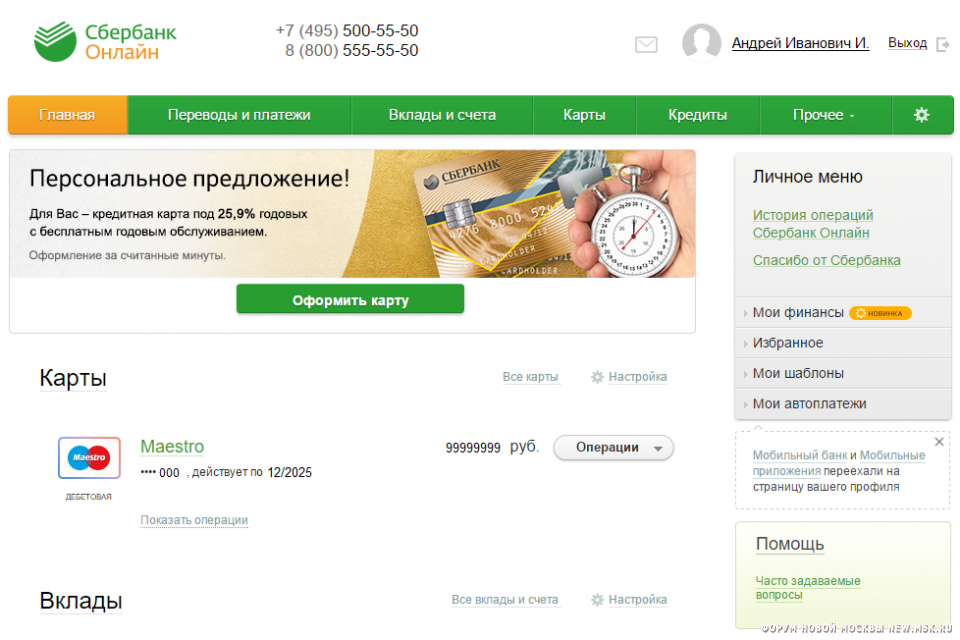
\includegraphics[width=5cm]{../pic/sber1.png}
	
\includegraphics[width=5cm]{../pic/sber2.png}
	
	\auditorium{Как будем решать эту задачу? Можно ли обойтись без нейронных сетей?
	Почему нейронные сети лучше не использовать?}
\end{frame}

\begin{frame}{Задача: определить бренд на одежде}
	\small
	Есть алгоритм С -- это краулер (уже разработан)
	Нужно разработать два алгоритма: А и B.
	А должен одежду (майки, кроссовки, штаны и т.д.),
	выделяя их из общей картинки. B должен на объекте обнаружить бренд.
	
	Цель -- защита от контрафакта: Avito, вК и т.д.
	
	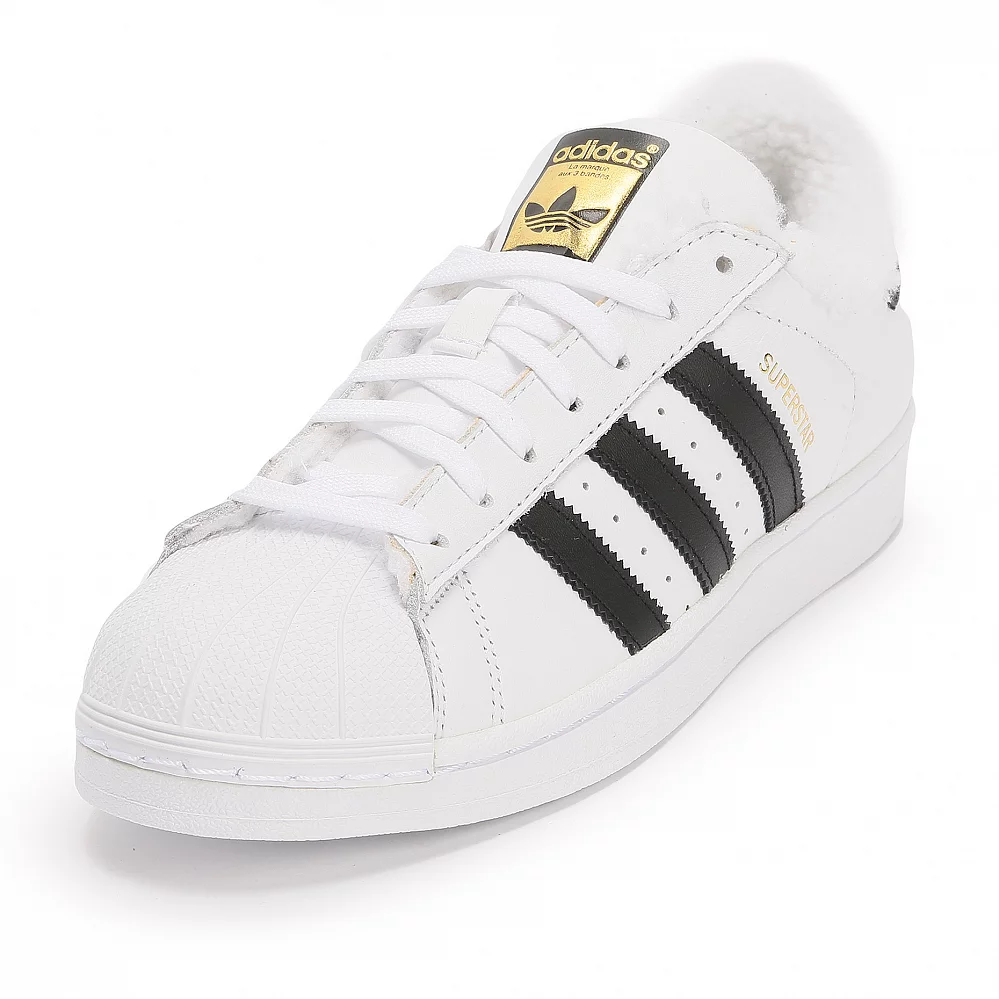
\includegraphics[width=4cm]{../pic/adidas1.png}
	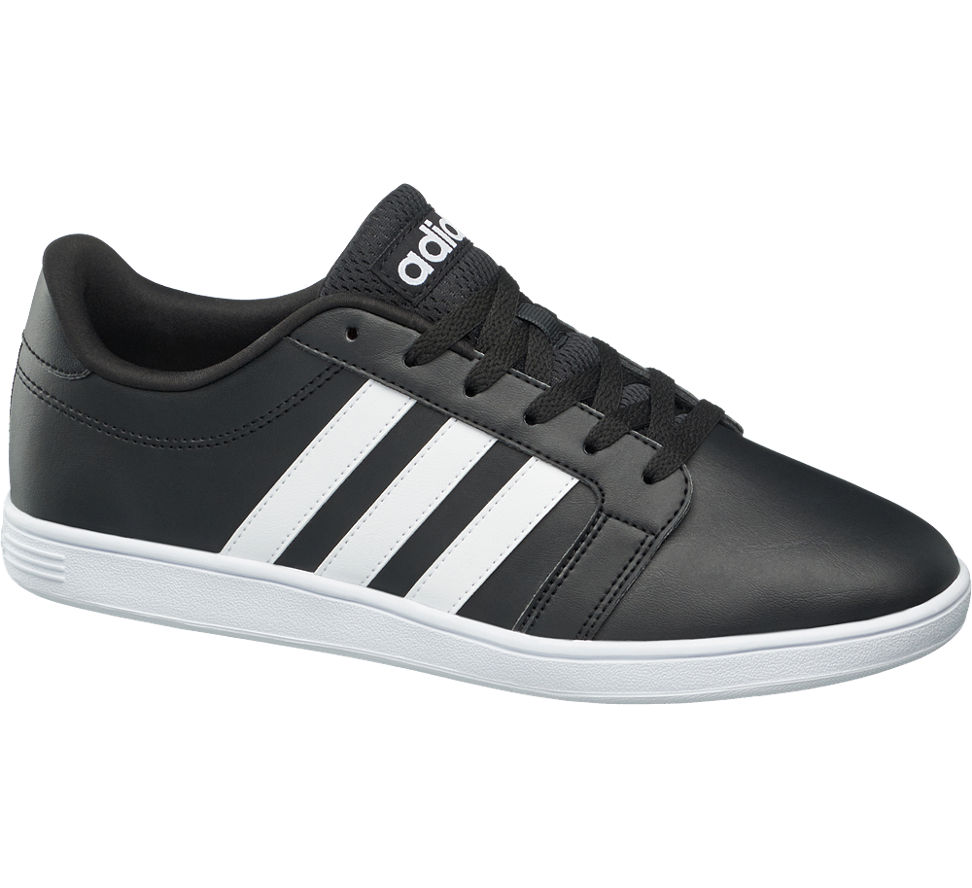
\includegraphics[width=4cm]{../pic/adidas2.png}
	
	
	\auditorium{Почему для данной задачи и A и B лучше решать
	с помощью нейронных сетей?}
\end{frame}

\begin{frame}{Предобученные нейронные сети}
	
	\begin{block}{Замечание}
	Сейчас уже нет необходимости обучать нейронку <<c нуля>>
	на протяжении нескольких недель на хороших серваках
	
	Уже есть библиотеки предобученных моделей. 
	Например: \url{https://keras.io/applications/}
	\end{block}
\end{frame}


\section{Feature Extraction в текстовых данных (Часть 1)}\label{section:texts_fe1}


\begin{frame}{Тексты и ИБ}
	Текстовая информация повсюду. 
	И может использоваться для ИБ задач
	\begin{enumerate}
		\item \auditorium{Примеры?}
	\end{enumerate}
\end{frame}


\begin{frame}{Тексты и ИБ}
	Текстовая информация повсюду. 
	И может использоваться для ИБ задач
	\begin{enumerate}
		\item Противодействие пиратству: описание фильмов
		\item Антиконтрафакт: описание продукции
		\item Даркнет: описание услуги/ВПО
		\item Фрод-мониторинг: СМС, назначение платежа, комментарий
		\item Анализ Трафик -- иногда его можно эффективно интерпретировать как текст
	\end{enumerate}
\end{frame}

\begin{frame}[fragile]{BoW}
	\termdef{BoW} (bag of words) -- множество с повторением, 
	основанное на тексте.
	
	Обычно BoW представляют в виде словаря вида:
	\begin{center}
		\texttt{\{"word": count\}}
	\end{center}
		
	Обычно процесс формирования BoW такой:
	\begin{enumerate}
		\item Поиск ресурса и получение документа (например HTML)

		\item Извлечение текста из документа
		\item Разбиение текста на \termdef{токены}. 
		Нормализация (Например \href{https://yandex.ru/dev/mystem/}{MyStem})
		\item Построение словаря: \href{https://docs.python.org/3/library/collections.html\#collections.Counter}{collectios.Counter}
	\end{enumerate}
\end{frame}

\begin{frame}{Что есть токен?}
	Самый простой способ задать токен -- это разбить на слова. 
	
	Но есть нюансы. Например единые понятия, состоящие из нескольких слов:
	<<морской огурец>>, <<цветная капуста>> и т.д.
	
	Так же есть языки, в которых не используются пробелы (китайский). 
	При этом само слово может состоять из многих графем. 
	(tǔ -- земля, dòu -- горох, tǔdòu -- картофель)
	
	\begin{block}{Замечание}
		Существуют задачи, в которых токенизация не является примитивной задачей
	\end{block}
\end{frame}

\begin{frame}{Нормализация токенов}
	Все токены следует нормализировать, привести к одной форме. 
	(для существительных -- единственное число, именительный падеж;
	для глаголов -- инфинитив и т.д.)
	
 	Бывают омонимы. Например "печь" -- это существительное или глагол?
	"мой" -- это от "мыть" или это местоимение?
	
	Будем считать омонимы -- \term{выбросами}.
\end{frame}

\begin{frame}{Закон Ципфа(Zipf)} 
	\small
	Возьмём очень большой \termdef{корпус}\footnote{\termdef{корпус}(линг.) -- совокупность текстов естественного языка}
	(Например все произведения Дарьи Донцовой)
		
	Обозначим за l количество слов в корпусе. $l >> 0$

	По оси $x$ отложим \termdef{шкалу порядка} слова.
	То есть упорядочим слова от самого употребляемого к самому неупотребительному.
	
	По оси $y$ -- количество раз, когда слово встречалось в тексте.
	
	Для любого естественного языка существует \termdef{гипербола} $g(x)$, такая что:
	\begin{equation}
	\lim_{l \longrightarrow \infty} \frac{y(x)}{g(x)} = 1
	\end{equation}
\end{frame}

\begin{frame}{Кривая Ципфа}
	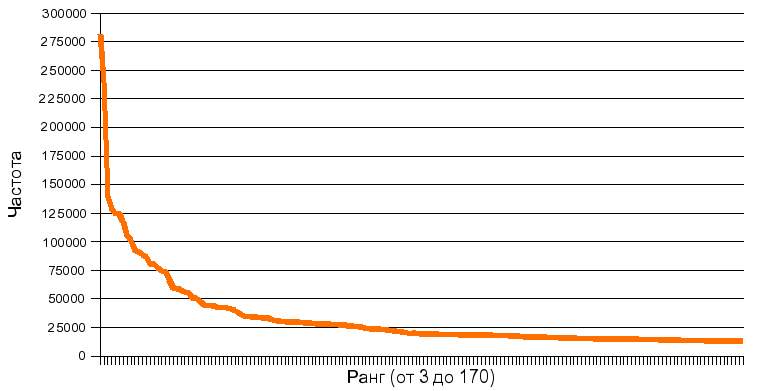
\includegraphics[width=11.5cm]{../pic/zipf_curve.png}
\end{frame}


\section{Алгоритм APTA}\label{section:APTA}


\begin{frame}{Алгоритм APTA}
	\termdef{APTA (AntiPiracy Text Analizer)} -- 
	очень простой и эффективный алгоритм, работающий
	в продукте \href{https://www.group-ib.ru/antipiracy.html}{Group-IB AntiPiracy}.
	
	\begin{block}{Замечание}
	Помимо APTA используется алгоритм APVI (AntiPiracy Video Identification) 
	-- анализатор видео-контента. 
	\end{block}
\end{frame}

\begin{frame}
	\begin{enumerate}
		\item 
		Возьмём корпус изучаемой нами задачи
		
		\begin{block}{Замечание}
		Очень важно взять корпус именно изучаемой задачи.
		Например если решаем проблему антипиратства, то корпус должен состоять 
		только из описаний к различным фильмам.
		\end{block}
		\item Для корпуса построим кривую Ципфа
		\item Разобьём ось $x$ на точки 
		\begin{equation}
		0 = x_0 < x_1 < x_2 < ... < x_n < x_{n+1} = \infty
		\end{equation}
		и зададим веса
		\begin{equation}
		0 = w_0 = w_1 < w_2 < w_3 < ... < w_n 
		\end{equation}
	\end{enumerate}
	... ... ...
\end{frame}

\begin{frame}
	\small
	\begin{enumerate}
		\item[4] Посчитаем предварительный скоринг ($preliminary\_score$) для каждого текста 
	\end{enumerate}
	
	Для этого для каждого текста $\bold t$ получаем его на токены (функция $get\_tokens$):
	\begin{equation}
		\left(t_1, t_2, ..., t_m\right) := get\_tokens (\bold t)
	\end{equation}
	
	Для каждгого токена определён его ранг: $x = x(t)$
	Задаём функцию скоринга для токена:
	\begin{equation}
	W(t) \stackrel{def}{=} w_i, ~\text{если}~ x_{i} \leqslant x(t) < x_{i+1}
	\end{equation}
	
	Тогда предварительный скоринг вычисляется по формуле:
	\begin{equation}
	preliminary\_score = -A(m) + \sum_{j=1}^{j=m} W(t_j)
	\end{equation}
	
	Функция $A(m)$ -- монотонно возрастающий от $m$ коэффициент
\end{frame}

\begin{frame}
	\begin{enumerate}
		\item [5]Зададим монотонно неубывающую функцию $\bold M$:
	\end{enumerate}
	
	\begin{equation}
	score \stackrel{def}{=} \bold M (preliminary\_score) \in [0, 1000]
	\end{equation}
	
	\auditorium{Как задать $\bold M$, если у нас есть тестовая выборка?}
	
	\auditorium{Как с помощью принципа $AI^2$ править функционал $\bold M$?}
\end{frame}


\begin{frame}
	Результат:
	\begin{itemize}
		\item Если исключить страницы, у которых вообще остуствует описание, то нет пропуска цели. Совсем
		\item Точность 98\%\footnote{По состоянию на июль 2018}. Но не всегда описание фильма -- это пиратство. Возможно 
		это фан-форум. \auditorium{Как решить эту проблему?}
		\item Нет описания фильма -- алгоритм не работает. Например это может быть переход по ссылке из объявления вК.
	\end{itemize}

\end{frame}

\section{Feature Extraction в текстовых данных (Часть 2)}\label{section:texts_fe2}

\begin{frame}{TF-IDF}
	\begin{itemize}
		\item TF — term frequency
		\item IDF — inverse document frequency
	\end{itemize}
	TF-IDF одна из самых старых \term{статистических} мер.
	Использовалась в поисковых системах выдачи в середине 90-х.
	
	\begin{equation}
	TF(t, \bold t) = \frac{count(t|\bold t)}{m(\bold t)}
	\end{equation}
	где $count(t|\bold t)$ -- 
	количество раз, когда токен $t$
	встречается в тексте $\bold t$;
	а $m(\bold t)=m$ -- это количество токенов в $\bold t$.
	
	% TODO
	
	
\end{frame}

\begin{frame}{Инструменты для работы с текстами}
	\begin{enumerate}
		\item
	\end{enumerate}

\end{frame}


\section{Вопросы для самопроверки}

\end{document}